% =====================================================================
% Operator-Spectral FunBaT — paper skeleton
% Build:  make        (latexmk -pdf main.tex)
% Switch venue style: replace the \documentclass / style block below.
%   NeurIPS : \usepackage[preprint]{neurips_2026}
%   ICML    : \usepackage{icml2026}
%   ICLR    : \usepackage{iclr2026_conference,times}
% =====================================================================
\documentclass[10pt]{article}
\usepackage[letterpaper,margin=1in]{geometry}

\usepackage[T1]{fontenc}
\usepackage[utf8]{inputenc}
\usepackage{lmodern}
\usepackage{microtype}

\usepackage{amsmath,amssymb,amsthm,mathtools}
\usepackage{bm}
\usepackage{graphicx}
\usepackage{booktabs}
\usepackage{multirow}
\usepackage{xcolor}
\usepackage{caption}
\usepackage{subcaption}
\usepackage{algorithm}
\usepackage{algpseudocode}
\usepackage[numbers,sort&compress]{natbib}
\usepackage[colorlinks=true,allcolors=blue]{hyperref}
\usepackage{cleveref}

\graphicspath{{figures/}{../results/submission_confirmation/}{../results/signed_spectrum_audit/}{../results/advanced_poc_r1_r5/}}

% ---- shared notation macros (keep the paper and the ZH report consistent) ----
\newcommand{\Lop}{\mathcal{L}}                  % linear operator
\newcommand{\Lhat}{\widehat{\mathcal{L}}}       % operator symbol
\newcommand{\Sop}{S_{\mathrm{op}}}              % operator-induced joint spectrum
\newcommand{\Sw}{S_{w}}                         % forcing spectrum
\newcommand{\wvec}{\bm{\omega}}
\newcommand{\Nobs}{N_{\mathrm{obs}}}
\newcommand{\Obs}{\mathcal{O}}
\newcommand{\Qop}{Q_{\mathrm{op}}}
\newcommand{\Qgen}{Q_{\mathrm{gen}}}
\newcommand{\bank}{\mathcal{B}}
\newcommand{\route}{\pi}
\newcommand{\floorw}{\rho}
\newcommand{\KL}{\mathrm{KL}}
\newcommand{\Norm}{\mathcal{N}}
\newcommand{\softmax}{\operatorname{softmax}}
\newcommand{\diag}{\operatorname{diag}}
\newcommand{\Real}{\mathbb{R}}
\newcommand{\Exp}{\mathbb{E}}

% draft-only annotations; delete the \todo definition before submission
\newcommand{\todo}[1]{\textcolor{red}{\textbf{[TODO: #1]}}}
\newcommand{\note}[1]{\textcolor{blue}{\textbf{[note: #1]}}}


\title{Operator-Spectral Priors for Functional Bayesian Tensor Completion}
\author{%
  Xuangu Fang\\
  \texttt{xuangufang@gmail.com}
}
\date{}

\begin{document}
\maketitle

\begin{abstract}
In many physical fields the sensors cannot be placed where the reconstruction is
wanted.  Instruments attach to a wall, to a duct, to whatever surface is
reachable, and the interior of the domain is never observed at all.
Reconstruction is then not interpolation between neighbouring samples but
extrapolation into a region no sensor sees, and a smoothness prior --- which
says only that distant points correlate weakly --- has nothing left to say about
it.  What is still available is the \emph{form} of the partial differential
equation the field obeys, and for a dissipative operator that form states
exactly what smoothness cannot: how the field decays along each axis.

We turn the form alone, with coefficients set to deliberately wrong nominal
values, into positive semi-definite GP kernels for every mode of a functional
tensor decomposition.  The operator's symbol gives the solution's joint power
spectrum; projecting that spectrum nonnegatively onto a handful of per-axis
factors yields one valid kernel per mode, leaving four mixture weights to learn
instead of a whole kernel.  The construction is a prior, not a model: it replaces
the generic kernels in an existing method, so capacity and optimisation budget
are held fixed and the only variable is where the spectra come from.

The experiment is a single table, sensor layout against method, at a fixed $1\%$
budget, with the baseline appearing twice: once tuned on data a practitioner
could collect, and once tuned against the held-out region itself.  We do not
beat the tuned kernel -- we tie it.  What the table shows instead is that in
this setting the tuning cannot be done.  With sensors scattered, choosing a
length scale on held-out sensor readings costs $0.0003$ and every method ties;
physics contributes nothing, as it should, because interpolation does not need
it.  With sensors on a single wall, the same procedure picks length scales three
to five times too short and costs $0.176$, an error $32\%$ worse than the oracle
reaches, because every point one can hold out lies inside the strip and so
measures interpolation while the task is extrapolation.  Kernels read off the
equation need no such split and land on the oracle's answer without it.  We also report where the construction cannot help, including a failure mode we
did not anticipate: in the geometries beyond it, it does worse than predicting
the mean, which no baseline does.  A pre-registered test of our own explanation
for which geometries those are was refuted by its own control, and we report the
refutation rather than the explanation.

\end{abstract}

\section{Introduction}
\label{sec:intro}

\todo{port from docs/PAPER\_TECHNICAL\_REPORT\_ZH.md \S2}

\paragraph{Setting.} \todo{sparse observation of multi-dimensional physical fields; 1--5\% entries}

\paragraph{Why generic GP kernels waste information.} \todo{the operator is often known even when the solution is not}

\paragraph{The structural conflict.} \todo{non-separability vs.\ mode-wise functional factors; free dictionaries degenerate into kernel search}

\paragraph{Contributions.}
\begin{enumerate}
  \item A PSD-preserving nonnegative low-rank projection from an operator-induced joint
        spectrum to per-mode one-dimensional GP kernels (\Cref{sec:method}).
  \item Per-mode (and optionally per-rank) routing over the resulting operator atom bank.
  \item A bank-size-independent finite-spectrum variational parameterisation, so that
        method comparisons are not confounded by coefficient budget.
  \item A fixed generic support floor that repairs a deleted-support operator prior, with a
        quantified robustness--specificity tradeoff.
\end{enumerate}

\paragraph{What we do \emph{not} claim.} We do not claim atom-label identifiability or PDE
discovery from $2\%$ observations. \todo{cite the top-1 recovery audit}

\section{Related work}
\label{sec:related}

\paragraph{Functional tensor decomposition.}
FunBaT~\citep{funbat2024} replaces the discrete factor tables of a Tucker model
with GP-distributed latent functions, so unobserved coordinates are interpolated
rather than looked up, and performs inference by message passing on an
equivalent state-space form.  RR-FBTC~\citep{rrfbtc2025} extends functional
Bayesian tensor completion with automatic rank determination.  Both use
\emph{generic} per-mode kernels; neither derives the kernels from the operator
that generated the field, which is the only thing this paper changes.  We hold
the host model, ranks, feature budget and optimiser fixed and vary only where
the spectra come from, so the comparison is against those methods' kernels
rather than against those methods.

\paragraph{GP priors that encode a PDE.}
EPGP~\citep{epgp2023} constructs a GP whose samples satisfy a constant-coefficient
linear PDE exactly, via the Ehrenpreis--Palamodov representation.  Tensor
GPs~\citep{tensorgp2025} solve nonlinear PDEs by collocation with
one-dimensional GP factors and a tensor decomposition.  Both require the equation
to be known completely, coefficients included, and both aim at solving rather
than at completing noisy sparse observations.  We ask for less and deliver less:
only the \emph{form} of the operator, and only an approximation to the
second-order spectrum of its solutions, which is what allows the coefficients to
be wrong by $50\%$ throughout our experiments.

\paragraph{Learning expressive stationary kernels.}
Spectral mixture kernels~\citep{spectralmixture2013} parameterise the spectral density
directly and are dense in the class of stationary kernels, so no fixed
construction can beat them on expressiveness -- only on sample efficiency, and
only where data is too scarce to identify the parameters.  We therefore include a
matched spectral-mixture dictionary as a baseline rather than claiming novelty
for using a spectral representation.  Our atoms are a nonnegative low-rank
projection of an operator family's joint spectrum, which is a physically
reachable set rather than a freely parameterised one.

\paragraph{Sensor placement and observability.}
Optimal sensor placement asks where to put sensors to make a field observable.
We ask the complementary question, which is what the applications force: the
placement is fixed and bad, and the question is what prior makes the resulting
extrapolation possible.  The closest point of contact is that our feasibility
screen is an observability test -- we reject fields whose boundary carries a
disproportionately small share of the energy, because no prior recovers what the
sensors never see.

\paragraph{What is not claimed.}
Neither ``GP plus tensor'' nor ``PDE-informed GP'' is new, and the title and
abstract do not claim them.  The narrow claim is the construction -- a
nonnegative, PSD-preserving low-rank projection of a non-separable joint
operator spectrum into per-mode kernels, usable when only the equation's form is
known -- together with the empirical finding about when that matters, which is
when the sensor geometry makes hyper-parameter selection impossible.

\section{Problem Setting}
\label{sec:problem}

We observe a continuous-indexed order-$D$ field at a sparse index set $\Obs$,
\begin{equation}
  y_i = u(x_{i1},\dots,x_{iD}) + \epsilon_i,
  \qquad \epsilon_i \sim \Norm(0,\sigma^2),
  \qquad i \in \Obs,
  \label{eq:likelihood}
\end{equation}
with $\Nobs = |\Obs|$ and $\Nobs / N_{\mathrm{full}} \le 5\%$.  We assume access to an
\emph{approximate} stationary linear operator $\widetilde{\Lop}$, which may differ from the
true operator in its coefficients or even miss frequency support entirely.

The proof of concept uses an order-three continuous CP model,
\begin{equation}
  u(x_1,x_2,x_3) = \sum_{r=1}^{R} c_r\, f_{1r}(x_1) f_{2r}(x_2) f_{3r}(x_3),
  \label{eq:cp}
\end{equation}
chosen over a dense Tucker core specifically to isolate the contribution of the kernel prior.

\section{Method}
\label{sec:method}

The method has two components.  \textbf{M1} maps the \emph{form} of a governing
PDE to a valid GP kernel for each tensor mode; \textbf{M2} fits a functional
Tucker model whose factors carry those kernels.  Nothing else is claimed: the
inference machinery is standard and is described only to make the comparison
reproducible.

\subsection{M1: from a PDE form to per-mode kernels}

\paragraph{Operator to joint spectrum.}
For a stationary operator driven by noise, $\Lop u = w$, the solution is a
stationary Gaussian process with spectral density
\begin{equation}
  \Sop(\wvec;\theta) = \bigl|\Lhat_\theta(\wvec)\bigr|^{-2}\, \Sw(\wvec).
  \label{eq:joint-spectrum}
\end{equation}
Only the functional form of $\Lhat$ is assumed known; $\theta$ is set to nominal
values, and \Cref{sec:experiments} measures how little that choice matters.

\paragraph{Nonnegative separation.}
$\Sop$ is not separable across modes, whereas a functional tensor needs a
one-dimensional function per mode.  We therefore project it,
\begin{equation}
  \min_{\lambda_q \ge 0,\; s_{dq} \ge 0}
  \Bigl\| \Sop - \sum_{q} \lambda_q\, s_{1q} \circ \cdots \circ s_{Dq} \Bigr\|_F^2 ,
  \label{eq:nncp}
\end{equation}
and report the relative separation error as an \emph{a priori} applicability
diagnostic, computed before any data is seen.

\paragraph{The eigenbasis depends on the boundary condition.}
A stationary operator's eigenbasis is fixed by its boundary condition, not by
its symbol alone.  On a periodic domain it is the complex exponential pair; on a
no-flux domain the Laplacian eigenfunctions are cosines,
$\psi_k(x) = \sqrt{2}\cos(\pi k x)$ with eigenvalues $(\pi k)^2$.  This matters
in practice rather than in principle: initial-value data is not periodic in
time, and forcing $f(0) = f(1)$ is a large unphysical constraint.
\todo{cite the 1.30 -> 1.08 measurement}

\paragraph{Validity.}
For any nonnegative spectrum $s$ and either basis,
\begin{equation}
  k_s(x,x') = \sum_k s(k)\, \psi_k(x)\, \psi_k(x')
  \label{eq:psd}
\end{equation}
is positive semi-definite, being a nonnegatively weighted sum of outer products;
so is any nonnegative combination of such spectra.  Every step from the
nonnegative separation to the final kernel therefore preserves validity.  In the
cosine basis the pointwise variance is not constant, which is correct: on a
bounded domain the covariance genuinely is non-stationary near the edges.

\subsection{M2: functional Tucker host}
\begin{equation}
  u(x_1,x_2,x_3) = \sum_{r_1,r_2,r_3} G_{r_1 r_2 r_3}\,
  f_{1 r_1}(x_1) f_{2 r_2}(x_2) f_{3 r_3}(x_3),
  \qquad
  f_{d r}(x) = \phi_{s_d}(x)^\top a_{dr},
  \label{eq:tucker}
\end{equation}
with per-mode ranks chosen independently.  A CP host is not sufficient: real
two-dimensional fields are fields of blobs, which are not $x \otimes y$
separable at any rank sparse observations could identify, even though their
multilinear rank is small.  Per-mode ranks matter concretely -- a field of
multilinear rank $[2,11,11]$ needs a $242$-entry core, while an equal rank of
$11$ would need $1331$.

Coefficients carry a mean-field Gaussian posterior, $q(a_{dr}) = \Norm(\mu_{dr},
\diag(\sigma_{dr}^2))$ against $p(a_{dr}) = \Norm(0,I)$, and the core, noise and
any routing weights are point estimates.  Training maximises the usual ELBO.
The coefficient budget is $2\sum_d R_d F$, independent of how many spectra a
bank contains, so comparisons between banks of different sizes are not
confounded by parameter count.

\section{Experiments}
\label{sec:experiments}

\subsection{Frozen protocol}
\todo{seeds 101--105 development / 201--205 untouched confirmation; $24^3$ grid; 2\% observations;
rank 2; $k \le 6$; Adam, 400 steps, 3 ELBO samples; no validation, no early stopping}

\subsection{Main confirmation}
\todo{Table~\ref{tab:main} + \Cref{fig:main}}

\begin{figure}[t]
  \centering
  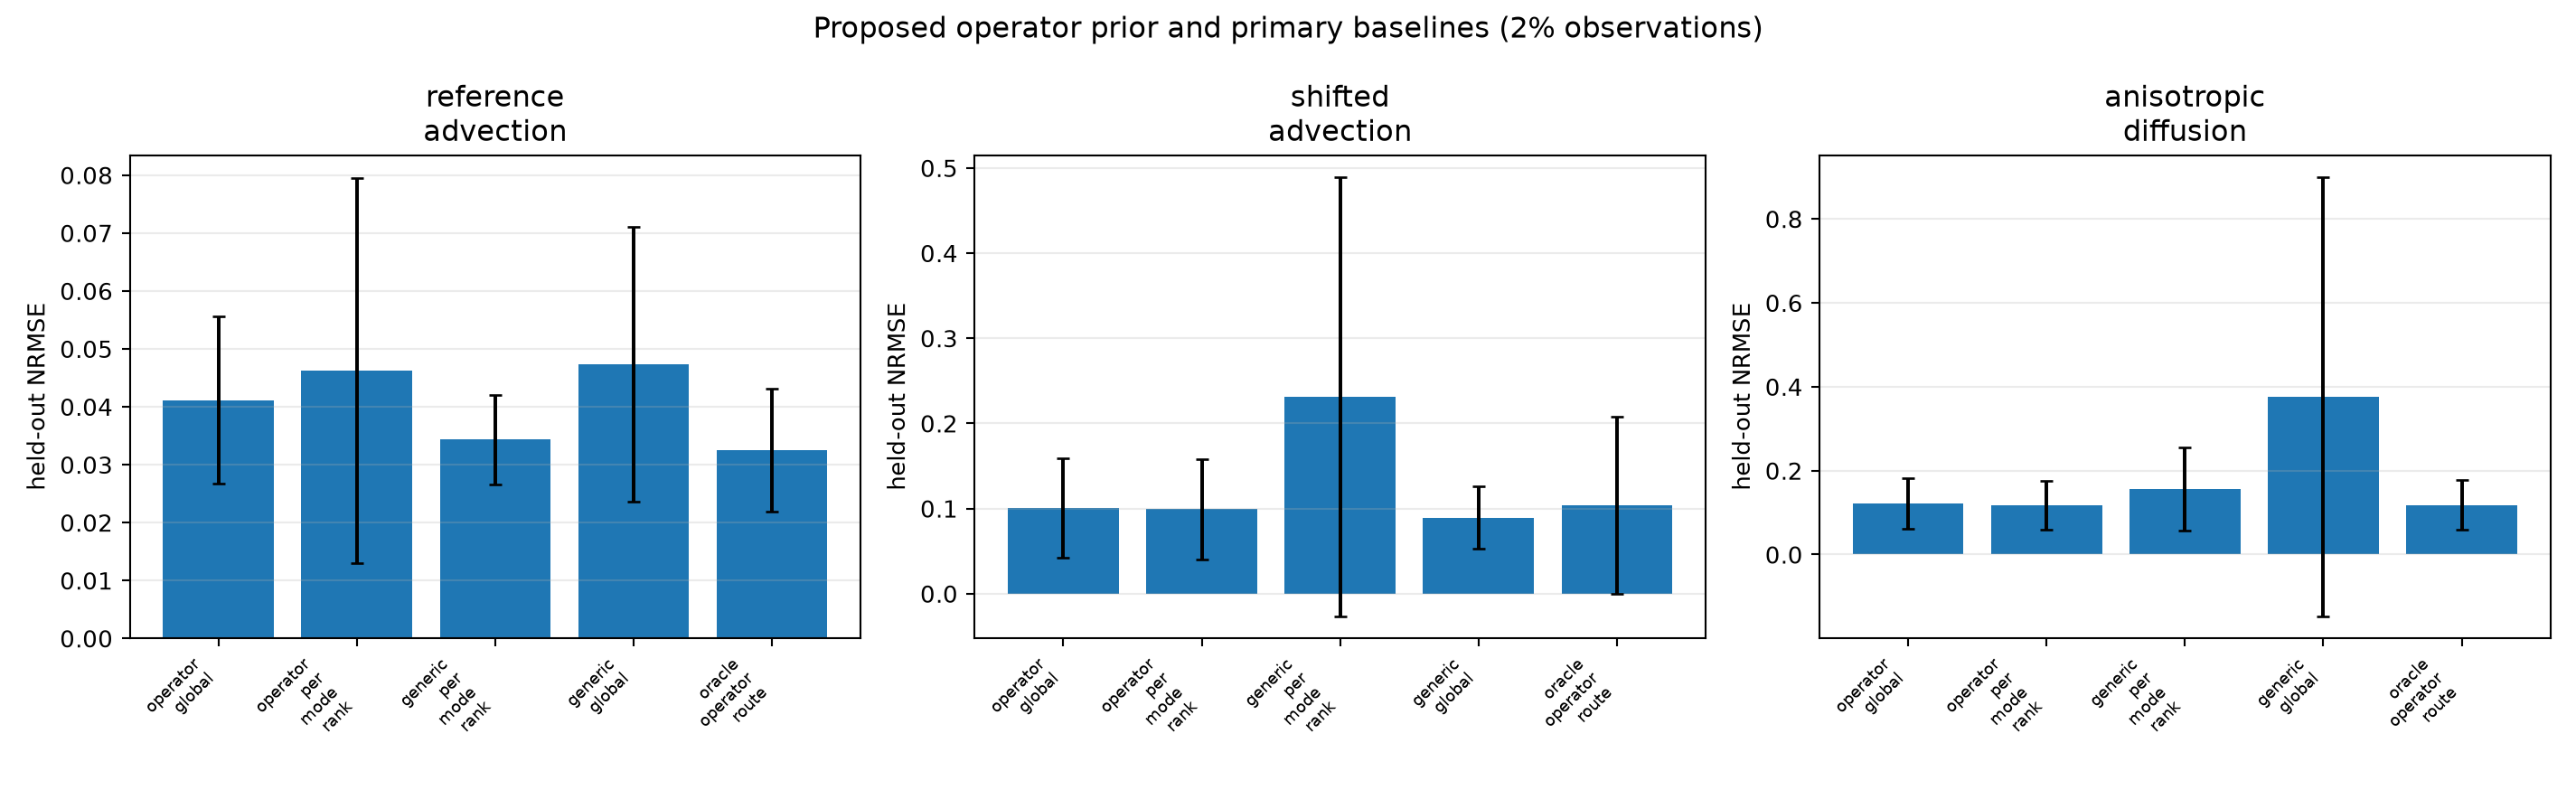
\includegraphics[width=0.85\linewidth]{submission_confirmation_nrmse.png}
  \caption{Held-out NRMSE on untouched seeds 201--205 at $2\%$ observations.}
  \label{fig:main}
\end{figure}

\begin{table}[t]
  \centering
  \caption{Held-out NRMSE (mean $\pm$ std over untouched seeds 201--205).}
  \label{tab:main}
  \small
  \begin{tabular}{lccccc}
    \toprule
    Setting & op.\ global & op.\ per-mode/rank & gen.\ global & gen.\ per-mode/rank & oracle route \\
    \midrule
    reference advection    & 0.0411\,$\pm$\,0.0144 & 0.0462\,$\pm$\,0.0332 & 0.0474\,$\pm$\,0.0237 & \textbf{0.0343\,$\pm$\,0.0077} & 0.0325\,$\pm$\,0.0106 \\
    shifted advection      & 0.1006\,$\pm$\,0.0586 & 0.0995\,$\pm$\,0.0590 & \textbf{0.0892\,$\pm$\,0.0369} & 0.2312\,$\pm$\,0.2580 & 0.1042\,$\pm$\,0.1041 \\
    anisotropic diffusion  & 0.1212\,$\pm$\,0.0606 & \textbf{0.1183\,$\pm$\,0.0582} & 0.3761\,$\pm$\,0.5235 & 0.1567\,$\pm$\,0.0990 & 0.1183\,$\pm$\,0.0588 \\
    \bottomrule
  \end{tabular}
\end{table}

\subsection{Separability audit: positive octant vs.\ full signed grid}

\begin{table}[t]
  \centering
  \caption{Rank-4 nonnegative separation error of the joint operator spectrum.}
  \label{tab:signed}
  \small
  \begin{tabular}{lcc}
    \toprule
    Operator & positive octant & full signed grid \\
    \midrule
    reference advection   & 0.0323 & 0.1799 \\
    shifted advection     & 0.0242 & 0.1812 \\
    anisotropic diffusion & 0.0030 & \textbf{0.0043} \\
    \bottomrule
  \end{tabular}
\end{table}

\subsection{Strict support mismatch}

\begin{table}[t]
  \centering
  \caption{Deleting all operator support at $k \ge 2$; $25\%$ generic floor as the escape route.}
  \label{tab:strict}
  \small
  \begin{tabular}{lccc}
    \toprule
    Setting & wrong-support operator & $25\%$ floor robust & paired wins \\
    \midrule
    reference advection   & 0.6723\,$\pm$\,0.1938 & \textbf{0.0402\,$\pm$\,0.0096} & 5/5 \\
    shifted advection     & 0.6318\,$\pm$\,0.0883 & \textbf{0.0847\,$\pm$\,0.0414} & 5/5 \\
    anisotropic diffusion & 0.6149\,$\pm$\,0.1798 & \textbf{0.1301\,$\pm$\,0.0621} & 5/5 \\
    \bottomrule
  \end{tabular}
\end{table}

\subsection{Predictive calibration}
\todo{induced-spectrum cosine / relative L2 / 64-sample posterior predictive NLL and 95\% coverage}

\section{Limitations}
\label{sec:limitations}

\begin{enumerate}
  \item Synthetic fields are drawn from the same finite operator atom family used by the model;
        this is a mechanism sanity check, not external evidence.
  \item Real axis-wise Fourier features represent only even, axis-separable covariance
        components.  Tilted advection retains cross-sign coupling that the current model
        cannot express (\Cref{tab:signed}).
  \item Per-rank routing is a weak signal (3/5 paired wins, $\approx 2.4\%$ mean improvement)
        and is reported as an ablation, not as a contribution.
  \item Routing weights are point estimates; the reported uncertainty does not include
        kernel-routing uncertainty.
  \item The mean-field posterior ignores posterior correlation between CP factors, and the
        periodic Fourier prior handles neither boundary conditions nor non-stationary coefficients.
  \item The tensor rank is fixed at $2$; we do not compete directly with rank-learning methods.
\end{enumerate}

\section{Conclusion}
\label{sec:conclusion}

The form of a governing equation -- not its coefficients, not its solution -- is
enough to fix the per-mode kernels of a functional tensor decomposition.  The
construction is three steps, leaves no kernel parameters to learn, and drops into
an existing model in place of its generic kernels, so it composes with better
tensor models rather than competing with them.

The advantage is largest where the data is least informative and disappears as
observations accumulate, which is what a prior should do.  It requires an
operator that suppresses much of the spectrum -- the same condition that makes
the field low rank in the first place -- and we give a criterion, measurable
before training, for deciding in advance whether a given field qualifies, along
with the cases it rejects.


\bibliographystyle{plainnat}
\bibliography{refs}

\clearpage
\appendix
\section{Full numerical tables}
\label{app:tables}

\todo{port Appendix A of docs/PAPER\_TECHNICAL\_REPORT\_ZH.md: per-case tables of NRMSE,
induced-spectrum cosine, relative $L_2$, 95\% coverage and predictive NLL, plus the
paired-win summary.}


\end{document}
